\documentclass[lang=cn,11pt]{elegantpaper}

\usepackage{multirow}

\title{使用博弈论和计算机模拟探讨社会规范对背叛现象的约束}
\author{赵鹏威\footnote{华中科技大学物理学院},U201710152,物理英才1701}

\begin{document}
	
	\maketitle
	
	\begin{abstract}
		\noindent 囚徒困境与它的变式在解释社会中的合作与背叛现象上已经取得了很好的成果,无论是在理论上,还是在计算机模拟上,都能够解释合作的产生机制和怎样才能抑制背叛行为。本文基于1986年 Axelrod 的计算机模拟,通过建立多阶段完全信息动态博弈,从理论上证明了计算机模拟结果的正确性。分析表明,在只具备社会规范的人类群体中,背叛现象不能得到抑制。当引入了对不愿意、拒绝惩罚背叛者的人予以谴责的元规范机制后,能够有效的抑制背叛现象的发生。另外,本文还使用遗传算法模拟了不具备理性假设的人类群体不断进行囚徒困境博弈的情况,模拟的结果显示随着人类群体的演化,背叛率会不断增加,并逐渐大于合作率,最后在一个较高的水平趋于稳定。
		\keywords{完全信息动态博弈,社会规范,计算机模拟,合作,背叛}
	\end{abstract}

\section{引言}\label{sec:引言}
囚徒困境是完全信息静态博弈的一个很典型的例子。囚徒博弈的解告诉我们,两个理性的博弈参与者在面对囚徒博弈时都会选择背叛对方。对每个博弈参与者来说,无论对方的选择是什么,他们选择背叛比选择合作得到的利益都要好。然而对于这两个人组成的整体来讲,如果他们都选择合作,那么两人的结果是最好的。实际生活中有很多囚徒博弈的例子,如石油的产量竞争。石油生产国总会经可能的多生产石油,试图获得更高的利益,但是他们这样做导致了石油价格下降,降低了他们的收益。而实际上,如果各个石油生产国能够合理地控制产量,他们就可以得到更多的收益。

从单次囚徒博弈中我们看到,理性的两人都是倾向于选择背叛。但是在现实生活中很显然存在合作的现象。实际上,如果重复多次或无限次囚徒博弈,就可以发现很多新的内容。从不少学者的研究看来,囚徒困境在解释社会中的合作现象如何产生和背叛现象怎样得到抑制的问题上已经取得了不少的成绩。Axelrod 在1981年发表的一篇文章\cite{axelrod1981evolution}中探讨了“在一个没有中央权威的自私世界里,合作要如何才能出现”这个问题,他指出,要想产生合作就必须是从长期看来合作的收益比背叛高。这之后,在 Axelrod 于1986年发表的另一篇论文\cite{Axelrod1986}中,Axelrod 使用计算模拟的方式研究了社会规范的作用,他的结果是仅仅靠对背叛者施加惩罚的社会规范(norm)无法抑制背叛现象的产生。他引入了元规范(metanorm)的概念,并得出元规范可以有效地促进合作抑制背叛现象的发生。所谓的元规范是指对看见有人背叛却不谴责他的人的谴责。除此以外,Axelrod 还在这篇文章中提出了抑制背叛现象的另外几种方法。Nowak Martin 和 May Robert 在1992年发表在 Nature 上的论文\cite{1992Nature}中指出如果人类群体分布的地域性,也可以产生合作现象。另外在他们还发现具有地域性的群体互相进行重复囚徒博弈,会出现与元胞自动机类似的现象,并且在一定条件下会出现混沌现象。

上面几位学者采用的研究方法主要是计算机模拟,而没有采用基于理性博弈参与者和共同知识假设的理论分析。这是由于他们考虑的博弈参与者的数量是巨大的,理论分析计算量太大。但是实际上,对于社会规范的作用,如果我们减少博弈参与者的个数,就可以使用博弈论的方法进行分析。在本文第\ref{sec:理论分析}节的讨论中会看到,这样做得出的结论与计算机模拟的结果是一致的。另外,在节\ref{sec:囚徒困境}中,通过计算机模拟的方式,又一次证明了,如果完全没有社会规范,即使参与者不是理性的,人们也会在进化的过程中选择背叛对方。


\section{理论分析}\label{sec:理论分析}
在这一节中,我们首先会参考 Axelrod 的论文\cite{Axelrod1986},给出社会规范和元规范的定义,然后分别构造一个完全信息动态博弈,这个博弈是多阶段重复的。我们将使用博弈树和子博弈精炼纳什均衡来求出博弈的解,并且阐述这个解对应的现实意义。

\subsection{社会规范下的博弈}
社会规范的定义又很多种,有基于行为的定义,基于期望的定义,也有基于价值的定义。本文采用 Axelrod 在论文\cite{Axelrod1986}中使用的定义,也是基于行为的定义:
\begin{quotation}
	社会规范指的是,在一定的社会背景下,社会中的多数人经常一定程度上按照某种方式行动,而被发现不按照这种方式行动的人经常会遭到其他人的谴责。
\end{quotation}
这个定义强调了“经常”,这是指社会中的人是否遵守规范和被发现违背规范时是否受到谴责是由概率控制的。为了便于理论分析的进行,可以做一些假设:
\begin{itemize}
	\setlength{\itemsep}{0.7ex}
	\item 一个人是否遵守规范不由概率控制,而由他自己决定;
	\item 只要一个人违反规范,他的行为就会被其他所有人发现;
	\item 一个人发现某人违反规范后是否谴责不由概率控制,而由他自己决定。
\end{itemize}
上面说的“自己决定”是说,博弈参与者按照理性和共同知识假设选择最优战略。

我们考虑的博弈分两阶段进行。第一阶段博弈中,每个参与者做出遵守规则或背叛规则的选择;第二阶段,博弈中,每个参与者选择是否惩罚(谴责)违反规则的人。下面我们将这个过程具体化:
\begin{itemize}
	\item 第一阶段:每个参与者都可以选择遵守或背叛。每有一个人选择背叛,那个人就会获得好处,他的支付就会增加$T$,而其他的人利益受到损害,支付会减少$H$;选择遵守的人对每个人的支付无贡献。
	\item 第二阶段:上一阶段每个参与者的选择成为共同知识。每一个参与者选择是否惩罚在第一阶段博弈中背叛的人(不能惩罚自己,因为这不合常理)。如果无人选择惩罚,则无事发生;如果选择惩罚,那么这个人需要付出一定的代价,每惩罚一个人,支付就减去$E$,而遭到惩罚的人将受到严厉的处理,支付减去$P$,但是受惩罚的人的支付最多减去$P$,不会因为有更多的人惩罚他而减去更多的支付。这里的$P$需要是一个相对较大的正数。
\end{itemize}
上面代表对支付的影响的量$T,\;H,\;E,\;P$都是正数。

在这个博弈中,每个参与者的战略应该包括两个方面。第一,战略要告诉参与者,在第一阶段博弈中是选择遵守还是选择背叛。第二,战略要告诉参与者,在已经看到第一阶段所有参与者的选择的情况下,是否选择惩罚背叛者,惩罚哪几个背叛者。

我们考虑一个最简单的情况,即只有两个人参与博弈。并且我们取$T=3,\;H=1,\;E=1,\;P=12$. 这样的一个二阶段博弈很方便用博弈树来表示。图\ref{fig:社会规范博弈树}就是这个博弈的博弈树。如果第一阶段两个人都选择遵守规范,那么博弈直接结束,两个人获得的支付都是$0$. 如果在第一阶段中有且只有一个人背叛,那么第二阶段时,之前遵守规则的那么人就可以选择惩罚另一个人,或是对对方的背叛保持沉默,如果选择惩罚,那么按照上面的说明,守纪者的支付为$-1-1=-2$,背叛者受到惩罚,支付为$3-12=-9$;若保持沉默,则守纪者只受到对方背叛带来的损失,支付为$-1$,而背叛者则维持背叛得到的好处,支付为$3$. 当两人都背叛时,在第二阶段中两人都可以选择是否惩罚对方,计算方法类似,不再赘述,只是说明一下当两人都背叛并都惩罚对方时,得到的支付$-11=T-H-E-P=3-1-1-12$.
\begin{figure}[htb]
	\centering
	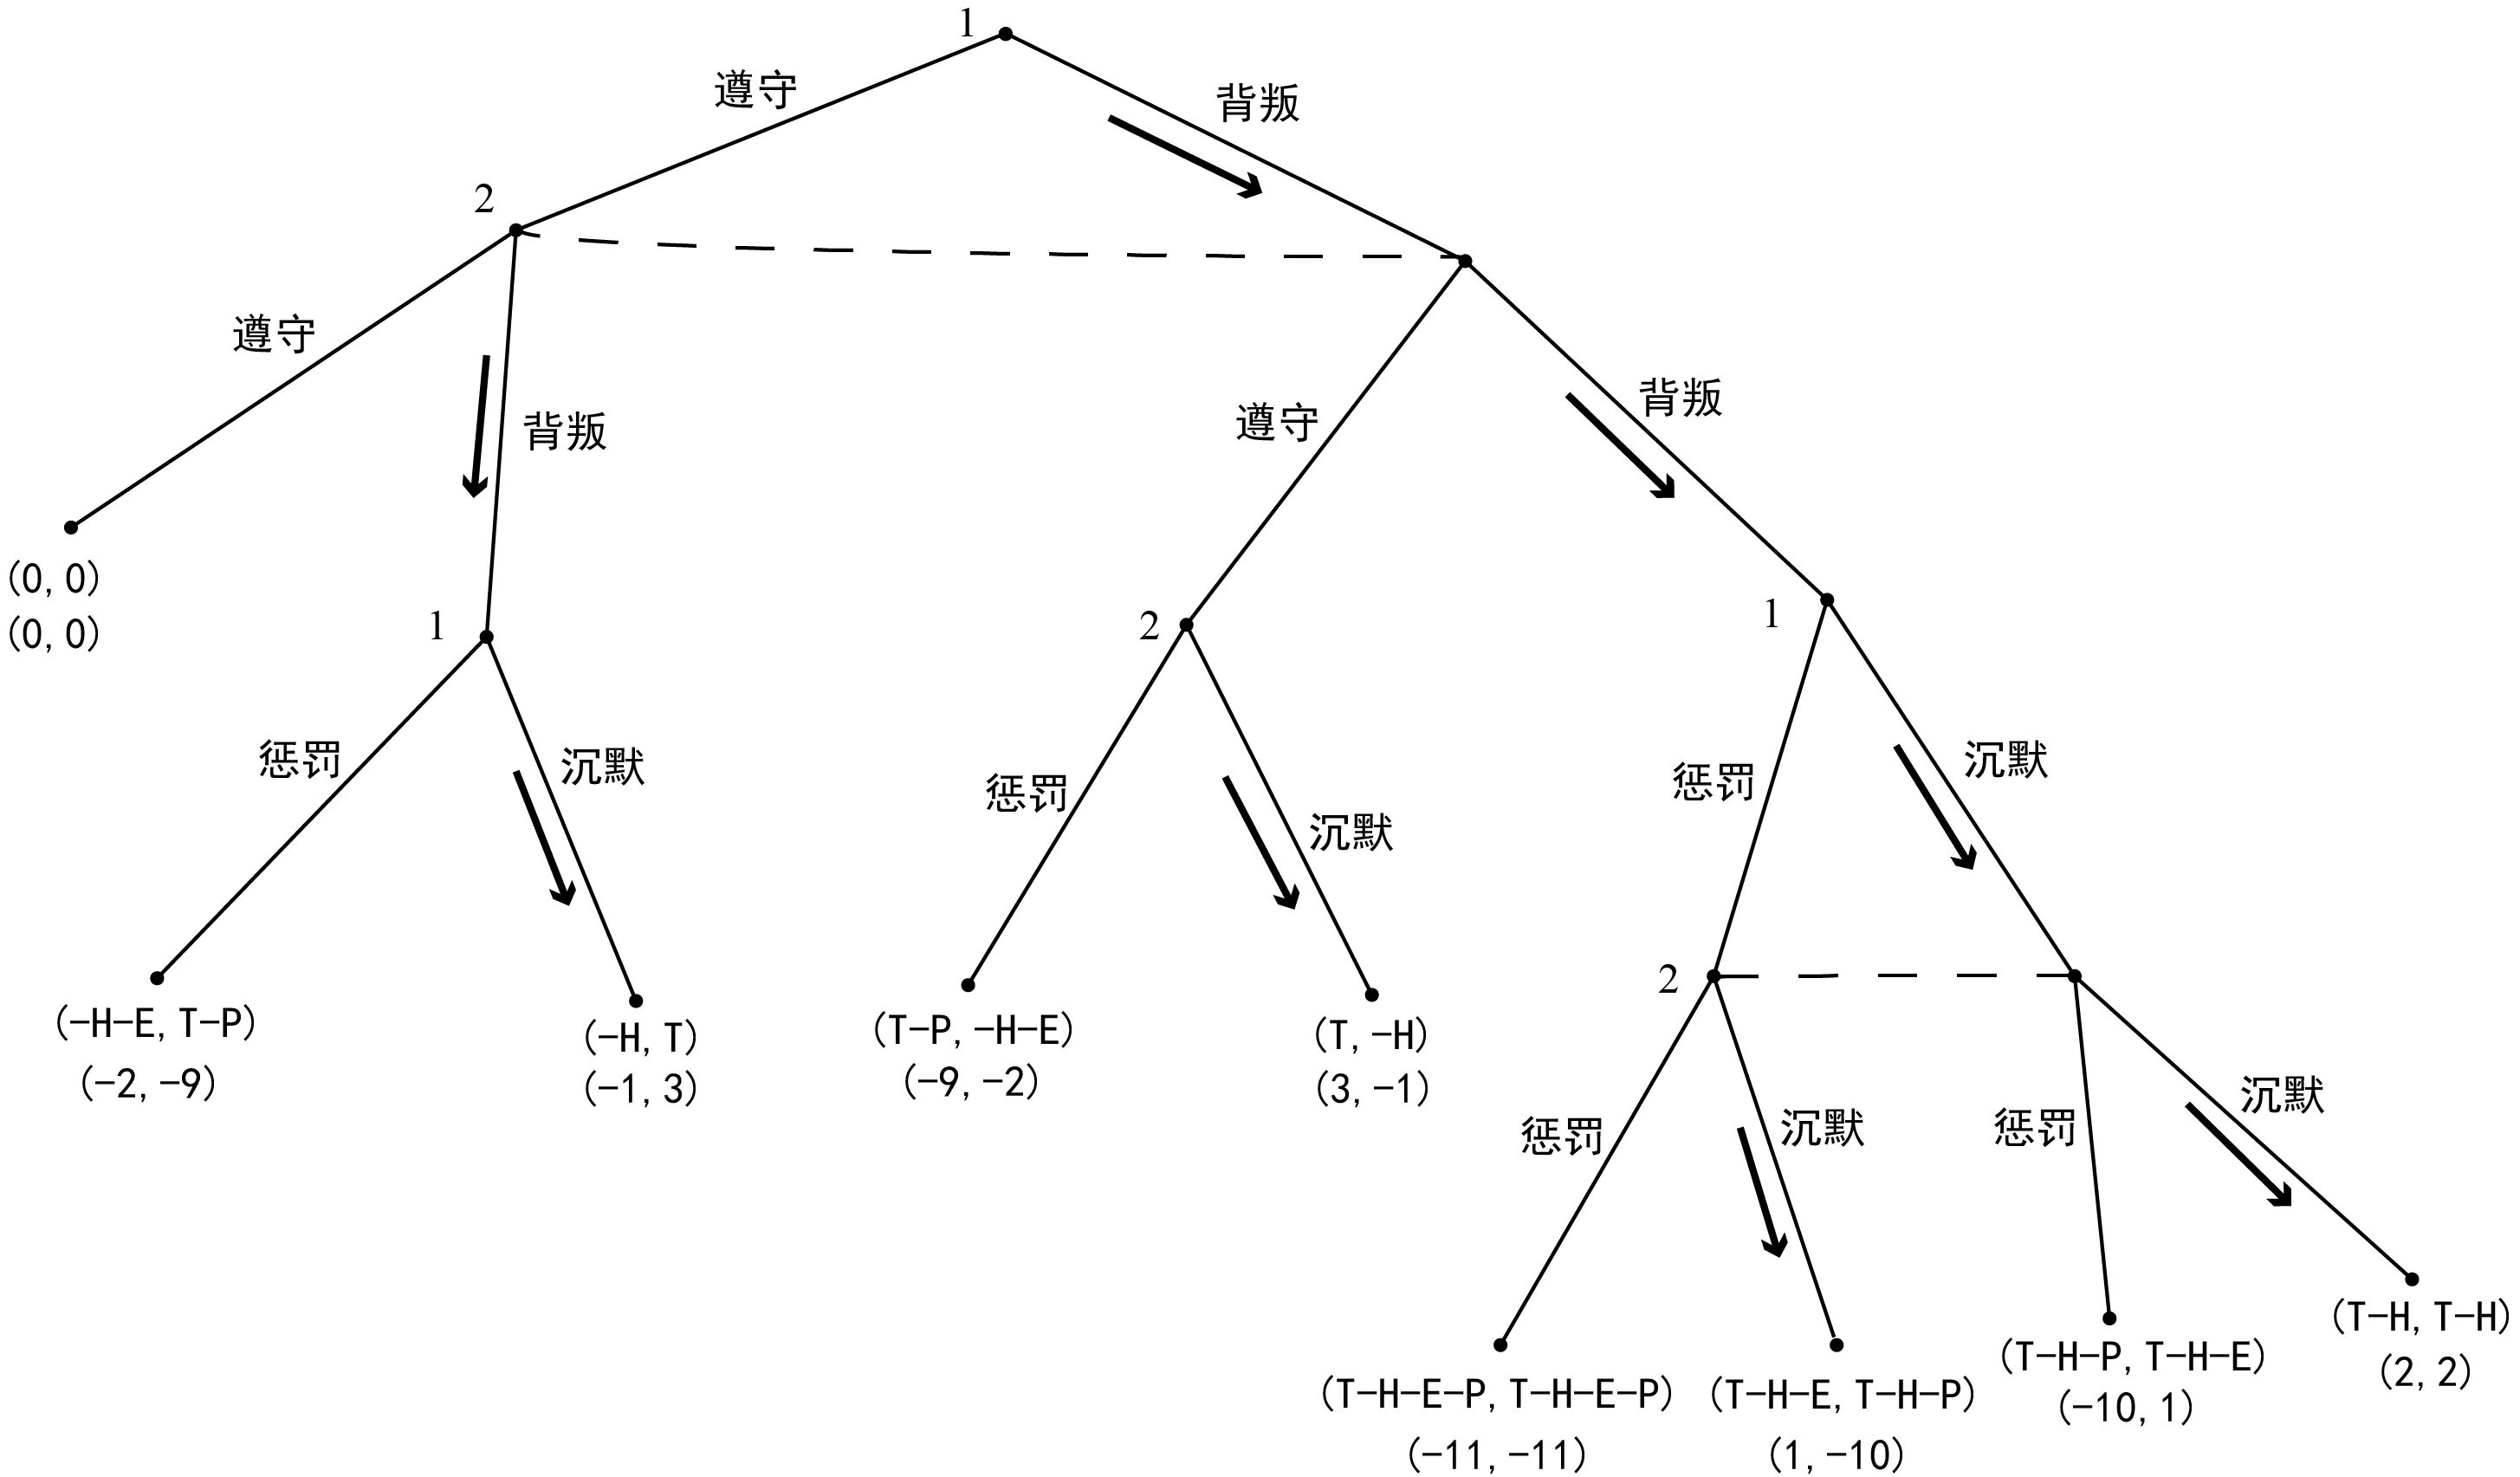
\includegraphics[width=0.8\textwidth]{figure/社会规范博弈树.png}
	\caption{考虑社会规范时的一种二阶段重复博弈,括号内的数值依次是参与者1和参与者2的支付,图中的箭头表示当参与者位于这个位置时会做出的选择。 \label{fig:社会规范博弈树}}
\end{figure}

我们用反向递推的方法来求这个博弈的解。可以发现位于每一个分支的最后一个节点的参与者无论是1还是2都会选择对对方的背叛保持沉默,因为如果选择惩罚对方,自己不会得到任何补偿,反而使自己的支付降低。对于第一阶段两者都背叛的情形,参与者1知道参与者2一定会选择沉默,那么他自己也会选择沉默,使自己得到$2$的支付而不是$1$. 这样我们知道了在第二阶段博弈中,无论时参与者1还是参与者2都会选择沉默,那么在第一阶段博弈中,两者自然就会都选择背叛。图\ref{fig:社会规范博弈树}的箭头表示的就是这个参与者在这个节点会做出的选择,可以看到,唯一的通路就是第一阶段两者都背叛,第二阶段两者都沉默。因此这种情况就是这个博弈的解,它是一个子博弈精炼纳什均衡。

上面的分析是基于$T=3,\;H=1,\;E=1,\;P=12$这一组特殊情况进行的,实际上对于一般的情况也是相同的结果。对于这样的一个具有社会规范的博弈,博弈论给出的答案是参与者在面对别人的背叛时,会保持沉默,不去惩罚背叛者,而且参与者都会选择背叛对方。可见,如果只存在惩罚背叛者的社会规范,是不能够抑制背叛现象的。导致这个结果最根本的原因是,惩罚对方不会让自己获得任何利益,反而需要付出更多的代价。另外一个方面是惩罚对方并不能挽回对方背叛造成的损失。背叛已经发生了,造成的结果已经成为了沉没成本,那么对于理性的参与者来说就没有必要惩罚背叛者,因为这样并不能挽回损失。因此,要想有效地抑制背叛现象的产生,就有两个方法。一个是让惩罚背叛者的人获得好处,比如补偿损失,或者给予奖励;另一个是给予对背叛者保持沉默的人谴责,迫使他们倾向于揭发背叛者的行为。

对于第一种方法,我们只需要在上述博弈中假定$E$是一个负数就可以发现,子博弈精炼纳什均衡只有可能是((遵守,遵守))和((背叛,背叛),(惩罚,惩罚))。而一般情况下,惩罚背叛者之后得到的好处不会很多,也就是说$T-H-E-P<0$,因此博弈的解就会是前一种情况,即所有人都遵守规则。可见,当惩罚背叛者可以获得好处时,理性的参与者都不再选择背叛,而是选择遵守规则。

第二种情况说的是如果某人对别人的背叛保持沉默,视而不见,那么需要有一种机制来谴责这样的人。这就是 Axelrod 在论文\cite{Axelrod1986}中引入的元规范(metanorm),我们将在下一节中利用博弈论分析这种情况。

\subsection{元规范下的博弈}
所谓元规范\cite{Axelrod1986},是指不仅惩罚那些背叛的人,而且还惩罚那些拒绝惩罚背叛者的人。据此,我们在上一节中的二阶段重复博弈后再添加一个阶段,这个阶段人们决定是否谴责上一阶段中拒绝惩罚背叛的那些人。我们考虑下面这个博弈:
\begin{itemize}
	\item 第一阶段:每个参与者都可以选择遵守或背叛。每有一个人选择背叛,那个人就会获得好处,他的支付就会增加$T$,而其他的人利益受到损害,支付会减少$H$;选择遵守的人对每个人的支付无贡献。
	\item 第二阶段:上一阶段每个参与者的选择成为共同知识。每一个在第一阶段中选择遵守的参与者选择是否惩罚在第一阶段博弈中背叛的人。如果无人选择惩罚,则无事发生;如果选择惩罚,那么这个人需要付出一定的代价,每惩罚一个人,支付就减去$E$,而遭到惩罚的人将受到严厉的处理,支付减去$P$,但是受惩罚的人的支付最多减去$P$,不会因为有更多的人惩罚他而减去更多的支付。
	\item 第三阶段:上一阶段每个参与者的选择成为共同知识。每一个在第二阶段中选择惩罚的参与者选择是否谴责在第二阶段博弈中选择沉默的人。被谴责者支付减去$P'$,谴责者的支付无变化。被谴责者的支付减少量是可以累加的。
\end{itemize}
注意这个博弈的第二阶段与上一节中考虑的博弈略有不同。上一节中背叛者也有资格惩罚别人,而这里不是,只有遵守规则的人才有资格惩罚别人。同样第三阶段中也是只有选择惩罚背叛者的人才有资格谴责保持沉默的人。

同样地,我们还是考虑一种特殊情况,即只有3个人参与博弈,取$T=3,\;H=1,\;E=1,\;P=12,\;P'=4$. 这样的一个博弈的博弈树是很庞大的,因此我们先从博弈树的一个分支出发。考虑表\ref{tbl:子博弈}所示的一个子博弈。
\begin{table}[htb]
	\centering
	\begin{tabular}{c|ccc}
		参与者 & 1 & 2 & 3 \\
		\hline
		第一阶段 & 遵守 & 背叛 & 遵守 \\
		第二阶段 & 惩罚 & 失格 & 沉默 
	\end{tabular}
	\caption{引入元规范后的博弈中的一个子博弈,“失格”表示参与者2没有资格参加第二阶段博弈。这之后参与者1需要选择是否谴责参与者3.\label{tbl:子博弈}}
\end{table}
现在参与者1面临选择,谴责参与人3还是不谴责。由于是否谴责对参与者1来讲没有区别,获得的支付是一样多的,因此这个这个子博弈的所有情况:谴责,不谴责,都是这个子博弈的纳什均衡。由于这个博弈只有3个参与者,不难发现到第三阶段最多只能有一人能够做出选择。我们假设每个参与者选择谴责的概率为$g$,再来考虑当第一阶段参与者1和3都选择遵守,参与人2选择背叛这个情况下的后续的博弈。这个子博弈可以用表\ref{tbl:收益矩阵}所示的收益矩阵来表示。
%\begin{table}[htb] 
%	\centering 
%	\begin{tabular}{cc|cc} 
%		& & \multicolumn{2}{c}{参与者1} \\
%		& & 惩罚 & 沉默 \\
%		\hline
%		\multirow{2}{*}{参与者3}& 惩罚 & (-3, -3) & (-3, -4g-1)  \\
%		& 沉默 & (-4g-1, -3) & (-1, -1)
%	\end{tabular} 
%	\caption{当第一阶段只有参与者2背叛时,博弈的收益矩阵,其中的$g$是每个参与者在第三阶段博弈中选择谴责的概率。\label{tbl:收益矩阵}} 
%\end{table}

\begin{table}[htb] 
	\centering 
	\begin{tabular}{c|cc} 
		& 参与者1惩罚 & 参与者1沉默 \\
		\hline
		参与者3惩罚 & (-3, -3) & (-3, -4g-1)  \\
		参与者3沉默 & (-4g-1, -3) & (-1, -1)
	\end{tabular} 
	\caption{当第一阶段只有参与者2背叛时,博弈的收益矩阵,其中的$g$是每个参与者在第三阶段博弈中选择谴责的概率。\label{tbl:收益矩阵}} 
\end{table}

如果$g<0.5$,那么$-4g-1>-3$,这时这个子博弈只有一个纳什均衡,即参与者1和3都沉默,获得支付$(-1,\;-1)$. 显然,这样的话,理性的参与者知道其他人在第二阶段博弈中不可能选择惩罚,那么他们在第一阶段博弈中为了利益最大化就会选择背叛。这样,这个博弈的解就是3个人都背叛,都获得1的支付。

如果$g>0.5$,这时表\ref{tbl:收益矩阵}所示的子博弈就会有两个纳什均衡,即两人都惩罚和两人都沉默。这样参与者1和3应该考虑混合战略,假设参与者1选择惩罚的概率为$p$,参与人2选择惩罚的概率为$q$,他们的混合战略分别是$(p,\;1-p)$和$(q,\;1-q)$. 混合战略均衡要求自己的选择带来的支付对对方的选择的期望要相等,因此可以列出下面的两个式子:
\begin{equation}
\left\{
\begin{split}
-3q-3(1-q)=(-4g-1)q-(1-q)\\
-3p-3(1-p)=(-4g-1)p-(1-p)
\end{split}
\right.
\end{equation}
可以解得:
\begin{equation}
p=q=\frac{1}{2g}>0.5
\end{equation}
可见两个参与者的混合战略是一样的,这是由这个博弈的对称性导致的。这个结果表明,在只有参与者2背叛的情况下,参与者1和3都选择惩罚的概率是$1/4g^2$,都选择沉默的概率是$(1-1/2g)^2<0.25$. 那么在第一阶段中,对参与者2来讲,如果他选择背叛,那么得到的支付的期望就是最多也只有$3*0.25-9*0.75=-6$. 不妨就用这个最大的支付期望来考虑第一阶段的博弈。这时第一阶段博弈也可以用收益矩阵表示,不过这是一个三维张量,为了方便,我们用A表示遵守,用B表示背叛,并把每种结果的支付用表\ref{tbl:收益矩阵2}表示每种情况的支付。
\begin{table}[htb] 
	\centering 
	\begin{tabular}{c|cccccccc} 
		选择 & (A, A, A)  &(A, A, B)& (A, B, A )& (B, A, A) & (A, B, B)  & (B, A, B)  & (B, B, A)  & (B, B, B)  \\
		\hline
		支付 &   (0, 0, 0)  &(-3, -3, -6)  & (-3, -6, -3)  &   (-6, -3, -3)  &   (-2, 2, 2)  &  (2, -2, 2)  &  (2, 2,-2)  &   (1, 1, 1) \\
	\end{tabular} 
	\caption{三个阶段的博弈可以等效成一个博弈,这个是这个博弈的支付。\label{tbl:收益矩阵2}} 
\end{table}

不难发现,有两个纳什均衡,一种是所有人都遵守,另一种是所有人都背叛。下面来考虑这个博弈的混合战略均衡。注意到这个博弈是完全对称的(对称是只任意次交换任意两个参与者,收益矩阵不变),那么这三个参与者的混合战略应该是一样的,那么可以假设每个参与者都有$r$的概率选择遵守。这样,可以列出下面的式子:
\begin{equation}
-3r(1-r)-3(1-r)r-2(1-r)^2=-6r^2+2r(1-r)+2r(1-r)+(1-r)^2
\end{equation}
解得$r\approx 0.66$,可见参与者选择遵守的概率要更大。而这个结论是在第二阶段中参与者选择沉默的概率为0.5,即$g=0.5$时得出的,当$g$增大时,参与者选择沉默的概率就会更小,因此在第一阶段博弈中他们就会越倾向于选择遵守规则。

通过上面的分析,我们看到只要$g>0.5$,或者说各个参与者都倾向于谴责那些对背叛者保持沉默的人,这时候参与者就会更可能选择遵守规则,而不是选择背叛。

\subsection{结论}\label{sec:结论}
从上面的分析我们看到,从简单的情况出发,利用博弈论的方法可以从理论上为 Axelrod 在论文\cite{Axelrod1986}中使用计算机模拟得到的结果提供合理的解释。理论分析的结果表明,一个社会如果只有惩罚背叛者的社会规范,并且这个惩罚行为需要施加惩罚的人付出一定的代价的话,那就和不具备社会规范的囚徒困境一样(在节\ref{sec:囚徒困境}中我会提供关于这个问题的计算机模拟结果),不能抑制背叛现象的发生,理性的参与者都会选择背叛其他人,让自己的利益最大化。想要抑制背叛现象,一方面,如果社会可以给施加惩罚的人提供好处,就有可能防止背叛的发生。另一方面,引入让拒绝惩罚的人得到利益损失的元规范,并且社会中的人都愿意谴责拒绝惩罚的人,或者说社会中的人具有恰当的正义感,他们会为面对背叛行为而保持沉默的人感到气愤,这样的话,也可以抑制背叛的发生。

理论的结果与 Axelrod 的模拟结果\cite{Axelrod1986}是一致的。在 Axelrod 的模拟中,只加入社会规范,经过多次博弈后,仍然有很多人会选择背叛。而当引入元规范时,背叛的人数就大大减少了,并且随着博弈次数的增加,选择背叛的人越来越少。

实际上,元规范在实际的社会中是普遍存在的。元规范的存在使得人们做出背叛、违规、违法等与社会向背离的行为的概率减小了,但是并不是完全减小到0. 显然现实中是存在背叛等现象的,这一点也与理论分析相符。

\section{计算机模拟}\label{sec:囚徒困境}
正如节\ref{sec:引言}和\ref{sec:结论}中提到的,大师 Axelrod 已经做过了有关社会规范等计算机模拟\cite{Axelrod1986}\cite{axelrod1981evolution},他的结果与本文利用博弈论的分析结果一致。这里就不再进行重复的工作了。下面我们通过遗传算法来模拟重复囚徒困境中合作与背叛的进化
\subsection{模型的建立}
囚徒博弈的收益矩阵在不同的文献里常常不同,因此为了下面的研究能够顺利进行,我们先规定本文所考虑的囚徒博弈:
\begin{quotation}
	囚徒博弈由两个参与者进行,两人不能交流。两人可以选择合作或者背叛。如果两个参与者都选择合作,那么他们将获刑2年;如果一人合作而另一人背叛,那么背叛的那个人将被释放,合作的那个人获刑5年;如果两个参与者都选择背叛,那么他们都将获刑5年。
\end{quotation}
我们规定被释放得到的收益为5,每多获刑1年,收益减去1. 这样,囚徒困境的收益矩阵可以表示如下:
\begin{table}[htb]
	\centering
	\begin{tabular}{c|cc}
		& A合作 & A背叛 \\
		\hline
		B合作 & 3, 3 & 5, 0 \\
		B背叛 & 0, 5 & 0, 0 \\
	\end{tabular}
	\caption{囚徒博弈的收益矩阵,每一格的第一个数字表示A的收益。数值越大代表得到的利益越好。}
\end{table}
博弈论的基本假设是理性假设和共同知识假设,这两个假设的存在确保了博弈问题的求解能够进行。但是,在现实生活中,这两个假设是非常强的假设,我们无法保证社会中的每一个个体都是完全理性的。如果社会中的每一个个体都是完全理性的,并且具有理性和游戏规则的共同知识,那么用纳什均衡作为博弈的解,一定会得到所有人都选择背叛这个结论。显然,这样对于我们研究人与人之间的信任的进化是没有帮助的。因此,我们抛弃这两个假设。另外,我们需要重复多次进行囚徒困境博弈。具体的过程如下:
\begin{quotation}
	我们将N次重复的囚徒困境博弈称作1次游戏。在一个人群中,每两个个体按照他们各自的战略进行一次游戏。这之后选出总收益最高的两人,使用他们的战略,按照既定的规则生成另一个人群,生成的人群中的个体再互相进行游戏。如此反复。
\end{quotation}

两人间的一次游戏就是N个相继进行的囚徒困境博弈,在每一次囚徒博弈中,参与者的选择要么是合作要么是背叛,如果我们用0表示合作,用1表示背叛,那么某个参与者的战略就可以用一个N位二进制数来表示。比如在5次相继进行的囚徒困境博弈,某个人的战略是“01101”,这就表示他在第一次博弈时选择合作,第二、三次博弈时选择背叛,第四次博弈时再选择合作,第五次博弈(也就是最后一次博弈)时选择背叛。这样的话,表示一个参与者就只需要两个参数:他的战略(一个N位二进制数)和他的总收益(或者称为得分)。

现在我们来定义如何通过两个个体生成一个新的人群。实际上只需要定义如何通过两个个体的战略生成另一个个体的战略就行了。为了模拟生物的遗传过程,我们按照下面的方式来从两个战略生成另一个战略:
\begin{itemize}
	\item 随机将这两者个体分为父本和母本
	\item 随机从同一个位置将父本的战略和母本的战略截断
	\item 将截断的父本战略的前一段与截断的母本战略的后一段拼接成一个新的战略
	\item 新的战略中的每一位分别按照既定的概率发生突变,0变成1,1变成0
	\item 利用上面得到的战略生成一个新的个体
\end{itemize}
这样,如果重复上面的过程,就可以从两个个体生成一个新的群体。比如有个体A和个体B,A的战略为10010,B的战略为01110,随机选择得到A为父本,B为母本,随机选一个位置,比如第2个,将战略截断,这样A的战略的前一段就是10,B的战略的后一段就是110,这两个战略片段合成为10110,作为新个体的战略。如果碰巧发生了突变,比如10110突变为了10010,那么新个体的战略就是10010了。需要注意的是每一次生成新个体时,谁是父本谁是母本和截断的位置都是需要重新随机选择的。
\subsection{计算机模拟结果}
模拟\footnote{本节中使用的程序使用 Python 编写,源代码已经上传到了 Github,如有需要,可以在\url{https://github.com/ZipWin/GameTheoryReaserch\_HUST}中找到}时设置的突变率为5\%,每一轮游戏包含1000次囚徒困境博弈,每一代人数为100. 进行100轮游戏。第一代初始化的战略全是0,即第一代只会选择合作。得到平均得分的进化曲线如图\ref{fig:分数进化曲线}所示。
\begin{figure}[!htb]
	\centering
	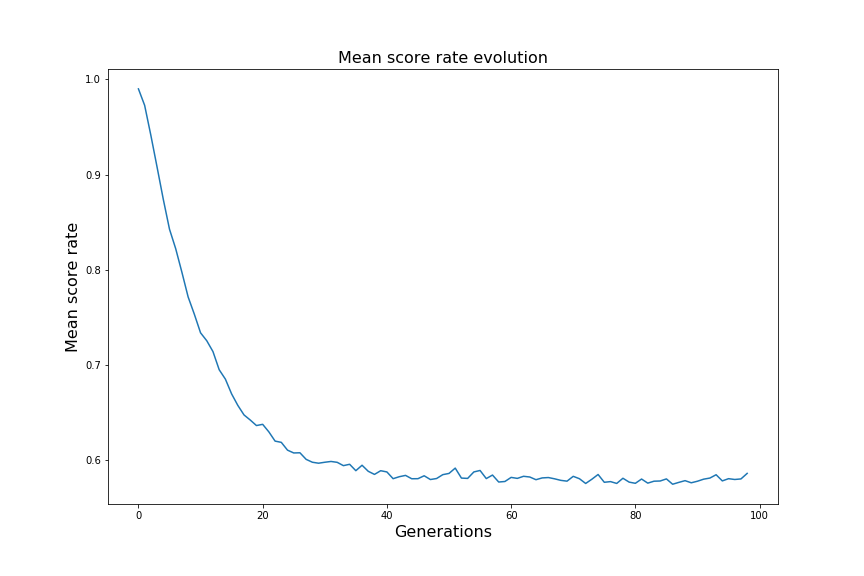
\includegraphics[width=0.8\textwidth]{figure/得分率的进化.png}
	\caption{进行100代游戏得到的平均得分进化曲线。平均得分指在每一代人中,每两个人进行一次游戏后,他们的得分的平均值。图中的纵轴表示的是平均得分占最大得分的比值,在本次模拟中最大得分时每次游戏包含的博弈数与每代人数的乘积再乘上3,即:$1000\times100\times3$. \label{fig:分数进化曲线}}
\end{figure}
可以看出,随着演化代数的增多,每一代的平均分数下降了。这并不是说明他们在演化中倒退了,因为实际上,随便选出一个后代与他们的祖先进行游戏,结果是后代的得分远远高于祖先。

另外,我们可以统计每一代人的战略中有多少次选择合作,有多少次选择背叛。得出的结果如图\ref{fig:信任进化曲线}所示。
\begin{figure}[!htb]
	\centering
	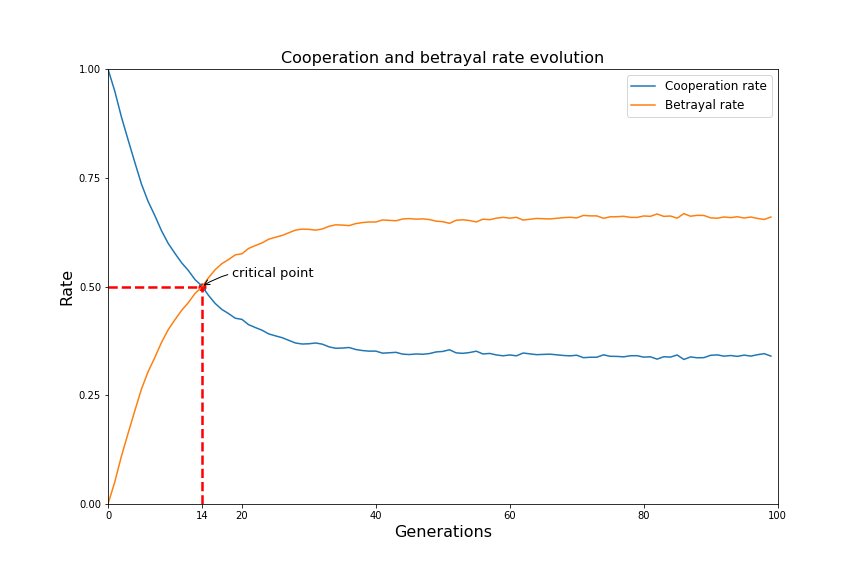
\includegraphics[width=0.8\textwidth]{figure/合作率的进化.png}
	\caption{ 每一代人的平均合作率和平均背叛率在100代演化过程中的变化,合作率即战略中0的个数占位数的比,背叛率即战略中1的个数占位数的比。图中递增的那条曲线是背叛率,递减的那条曲线是合作率,两条曲线相交于点 (14, 0.50).\label{fig:信任进化曲线}}
\end{figure}
从图\ref{fig:信任进化曲线}中可以看出,随着演化的进行,每代人的合作率逐渐下降,背叛率逐渐上升。这个结果表明,在抛弃理性假设的情况下,完全让人群根据他们得到的利益大小演化,得到的结果也是背叛发生的概率越来越高。与博弈论的结果具有一致性。

另外,从图\ref{fig:信任进化曲线}还可以得到一个信息,即当演化的代数足够多时,合作率和背叛率会趋于稳定,两者的极限值分别约为0.35和0.65. 可见,虽然演化中背叛率会上升,并不会有完全背叛的人出现。实际上最强的战略应该时全为1,即完全背叛。模拟中没有出现完全背叛是由突变率决定的,由于突变率设置的是5\%,而战略一共有1000位数字,想要从演化的稳定状态,即背叛率为0.65突变成背叛率为1.00,这个概率是$0.5^{350}$,这显然是几乎不可能发生的。但是反过来,如果我们在初始化第一代时将他们的战略全都设置为完全背叛,那么无论演化多少代,模拟的结果都会是背叛率一直稳定在1.00.

\section*{补充的话语}
本文使用\LaTeX 编写,论文的源代码和模拟重复囚徒困境的Python代码已经上传到了\url{https://github.com/ZipWin/GameTheoryReaserch\_HUST},如有需要可以查看。本文的灵感来源于课程上所讲的使用重复囚徒困境来解释社会中的合作与背叛现象的内容。另外,还参考了梅拉妮·米歇尔所著的《复杂》的第14章
\cite{complex},"metanorm" 的中文译文“元规范”也是参考这本书的。在博弈论的基本理论方面,还参考了 Robert Gibbons 的《博弈论基础》前2章\cite{game}.

\bibliographystyle{plain}
\bibliography{wpref}

\end{document}